\documentclass{beamer}

\usepackage{beamerthemesplit}
\usetheme{Singapore} %Copenhagen}
%\usecolortheme{whale}

\beamertemplatenavigationsymbolsempty % Hide navigation panel

\usepackage[T2A]{fontenc}
\usepackage[utf8]{inputenc}
\usepackage[russian]{babel}


\usepackage{textcomp}
\usepackage{amssymb,amsmath}
%\usepackage{animate}
%\usepackage{longtable}
\usepackage{xcolor}

%\usepackage{pstricks}

\newcounter{N}

%% Форматирование окружения itemize
%\usepackage{ragged2e}
%\let\olditem\item
%\renewcommand\item{\olditem\justifying}


\title[]{Дивергенция и ротор векторного поля}

\author[]{ {\em Верещагин Антон Сергеевич}
	\\
	канд. физ.-мат. наук, доцент\\
	\bigskip
	Кафедра аэрогидродинамики ФЛА НГТУ
}

\newtheorem{dfn}{Определение}  
\newtheorem{theorems}{Теорема}  

\newcommand{\Rn}{\mathrm{R}^n}
\newcommand{\Sm}{\mathrm{S}^m}
\newcommand{\Ql}{\mathrm{Q}^l}

\newcommand{\Rd}[1]{\mathbb{R}^{#1}}
\newcommand{\Vn}{\mathrm{V}^n}

\newcommand{\oper}[1]{{\bf #1}}
\newcommand{\basis}[1]{\vec{\bf #1}}
\newcommand{\dt}[1]{\frac{d #1}{dt}}
\newcommand{\dtds}[1]{\displaystyle\frac{d #1}{dt}}
\newcommand{\ds}[1]{\frac{d #1}{ds}}
\newcommand{\dsds}[1]{\displaystyle\frac{d #1}{ds}}
\newcommand{\dsd}[1]{\frac{d^2 #1}{ds^2}}
\newcommand{\pdt}[1]{\frac{\partial #1}{\partial t}}
\newcommand{\pds}[1]{\frac{\partial #1}{\partial s}}
\newcommand{\pdx}[1]{\frac{\partial #1}{\partial x}}
\newcommand{\pdy}[1]{\frac{\partial #1}{\partial y}}
\newcommand{\pdz}[1]{\frac{\partial #1}{\partial z}}
\newcommand{\pdxds}[1]{\displaystyle\frac{\partial #1}{\partial x}}
\newcommand{\pdyds}[1]{\displaystyle\frac{\partial #1}{\partial y}}
\newcommand{\pdzds}[1]{\displaystyle\frac{\partial #1}{\partial z}}
\newcommand{\pdn}[1]{\frac{\partial #1}{\partial n}}
\newcommand{\grad}[1]{{\rm grad}\, #1}
\newcommand{\gradvds}[1]{\basis{i}\pdxds{#1}+\basis{j}\pdyds{#1}+\basis{k}\pdzds{#1}}

\newcommand{\dv}[1]{\operatorname{div}\vec{#1}}
\newcommand{\dvdef}[1]{\pdx{#1_x}+\pdy{#1_y}+\pdz{#1_z}}
\newcommand{\dvwv}[1]{\operatorname{div} #1}
\newcommand{\rot}[1]{\operatorname{rot}\vec{#1}}
\newcommand{\rotpr}[2]{\operatorname{rot}_{#1}\vec{#2}}
\newcommand{\rotwv}[1]{\operatorname{rot} #1}

\begin{document}

\frame{\titlepage}


\frame{
\frametitle{Аннотация}
\parbox{\textwidth}{Дивергенция вектора. Теорема Гаусса-Остроградского. Ротор вектора. Теорема Стокса и ее следствия.
}
}


\frame{
\frametitle{Поток вектора через поверхность}

\begin{columns}
\begin{column}{0.6\textwidth}
\begin{dfn}
\parbox{\textwidth}{
Интеграл, определенный для площадки $S$, \pause над векторным полем $\vec{a}$ как предел  \pause 
\[ 
\displaystyle\int\limits_S\vec{a}\cdot d\vec{S}= \pause 
\lim\limits_{\Delta S_j\rightarrow 0}\sum\limits_j\vec{a}_j\cdot\Delta \vec{S}_j,
\] \pause 
}
\end{dfn}
\end{column}
\begin{column}{0.4\textwidth}
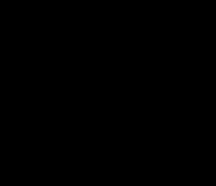
\includegraphics[width=\textwidth]{../img/vector_flow.png}
\end{column}
\end{columns}
\parbox{\textwidth}{\it
называется \alert{потоком вектора} $\vec{a}$ через поверхность $S$. \pause 


\medskip
Здесь $\Delta S_j$ -- элементарные площадки разбивающие поверхность $S$;  \pause 
$\vec{n}_j$ -- внешняя единичная нормаль в любой точке $\Delta S_j$; \pause 
$\vec{a}_j$ -- значение векторного поля $\vec{a}$ в любой точке площадки $\Delta S_j$;  \pause 
$\Delta\vec{S}_j=\vec{n}_j\Delta S_j$.
}
}


\frame{
\frametitle{Дивергенция вектора}
\begin{columns}
\begin{column}{0.4\textwidth}
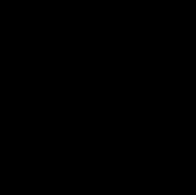
\includegraphics[width=\textwidth]{../img/divergence.png} \pause 
\end{column}
\begin{column}{0.6\textwidth}
\begin{dfn}
\parbox{\textwidth}{
\alert{Дивергенция вектора} $\vec{a}$ в точке $P$  \pause есть отнесенный к единице объема $V$ поток вектора $\vec{a}$ через поверхность $S$,  \pause окружающую точку $P$, при стягивании последнего в точку $P$: \pause 
}
\end{dfn}
\end{column}
\end{columns}

\parbox{\textwidth}{

\bigskip
\[ 
\dv{a}=
\lim\limits_{V\rightarrow 0}\frac{1}{V}\int\limits_S \vec{a}\cdot\vec{n}dS=
\lim\limits_{V\rightarrow 0}\frac{1}{V}\int\limits_S a_n dS.
\]
}

}

% Добавить вывод дифференциального представления дивергенции
%\frame{
%\frametitle{}
%}

\frame{
\frametitle{Представление дивергенции в дифференциальной форме}
\parbox{\textwidth}{
Если разложить функцию $\vec{a}=a_x\basis{i}+a_y\basis{j}+a_z\basis{k}$ в окрестности точки $P$, тогда 
\alert{
\[
\dv{a}=\dvdef{a}.
\]
} \pause 

\bigskip
С использованием оператора Гамильтона (наблы):
\alert{
\[
\dv{a}=\nabla\cdot\vec{a},
\]
}
\[
\nabla=\gradvds{}.
\]
} 
}

\frame{
\frametitle{Теорема Гаусса-Остроградского}
\begin{theorems}[Гаусса-Остроградского]
\normalfont
\parbox{\textwidth}{
Поток вектора через замкнутую поверхность равен объемному интегралу от дивергенции вектора: \pause 
}
\end{theorems}
\begin{columns}
\begin{column}{0.5\textwidth}
\[ 
\int\limits_S \vec{a}\cdot\vec{n} dS=\int\limits_V\dv{a}dV.
\] \pause 
\end{column}
\begin{column}{0.5\textwidth}
\centering
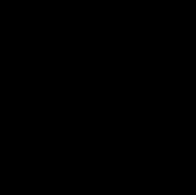
\includegraphics[width=0.8\textwidth]{../img/gauss_ostr_illustr.png}
\end{column}
\end{columns}
}

\frame{
\frametitle{Теорема Гаусса-Остроградского}
\begin{proof}
\end{proof}
}

%\frame{
%\frametitle{Вывод уравнения неразрывности}
%}

\frame{
\frametitle{Соленоидальное векторное поле и его свойство}
\begin{dfn}
\parbox{\textwidth}{
Векторное поле $\vec{a}$, для которого во всех точках справедливо равенство $\dv{a}=0$,  называется \alert{соленоидальным}.  
}
\end{dfn} \pause 

\begin{theorems}
\normalfont
\parbox{\textwidth}{
Для соленоидального вектора его поток через любое поперечное сечение векторной трубки тока имеет одну и ту же величину.
}
\end{theorems}
}


\frame{
\frametitle{Соленоидальное векторное поле и его свойство}
\begin{proof}
\parbox{\textwidth}{
\includegraphics[width=0.7\textwidth]{../img/solenoid.png} \pause 
\[
0=\int\limits_V\dv{a}dV= \pause 
\int\limits_{\Sigma}\vec{a}\cdot\vec{n}dS= \pause 
\int\limits_{\Sigma_1}\vec{a}\cdot\vec{n}_1 dS+
\int\limits_{\Delta\Sigma}\vec{a}\cdot\vec{n}_\Delta dS+
\int\limits_{\Sigma_2}\vec{a}\cdot\vec{n}_2 dS.
\] \pause 
Отсюда  $\int\limits_{\Sigma_1}\vec{a}\cdot\vec{n}_1 dS=-\int\limits_{\Sigma_2}\vec{a}\cdot\vec{n}_2 dS$, \pause 
т.к. $\int\limits_{\Delta\Sigma}\vec{a}\cdot\vec{n}_\Delta dS=0$ в силу ортогональности векторов $\vec{a}$ и $\vec{n}_\Delta$,  \pause т.е. потоки вектора $\vec{a}$ через $\Sigma_1$ и $\Sigma_2$ совпадают.
}
\end{proof}
}

\frame{
\frametitle{Циркуляция вектора по замкнутому контуру}
\begin{dfn}
\parbox{\textwidth}{
\alert{Циркуляцией  вектора} $\vec{a}$ по замкнутому контуру называется следующий интеграл (с выбранным направлением интегрирования): \pause 
\[ 
\Gamma_C(\vec{a}) = \int\limits_C\vec{a}\cdot d\vec{r}.
\]
}
\end{dfn}

}

\frame{
\frametitle{Ротор вектора}

\begin{dfn}
\parbox{\textwidth}{
Выберем плоскую площадку $S$, содержащую точку $P$, с нормалью $\vec{n}$ и контуром $C$,  \pause тогда \alert{ротором в направлении $\vec{n}$} в точке $P$ называется отношение циркуляции вектора по контуру $C$ к площади $S$, когда последняя стягивается в точку $P$: \pause 
}
\begin{columns}
\begin{column}{0.4\textwidth}
\centering
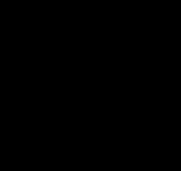
\includegraphics[width=0.8\textwidth]{../img/rotor.png} \pause 
\end{column}
\begin{column}{0.6\textwidth}
\[ 
\rotpr{\vec{n}}{a}=\lim\limits_{S\rightarrow 0}\frac{\int\limits_C\vec{a}\cdot d\vec{r}}{S}
\]
\end{column}
\end{columns}

\end{dfn}

}

% Добавить вывод дифференциального представления ротора
%\frame{
%\frametitle{}
%}

\frame{
\frametitle{Дифференциальное представление ротора}
Если представить $\rotpr{\vec{n}}{a}$ в дифференциальной форме по трем основным направления, \pause тогда
\alert{
\[ 
\rotpr{x}{a}=\pdy{a_z}-\pdz{a_y},\quad \rotpr{y}{a}=\pdz{a_x}-\pdx{a_z},\quad \rotpr{z}{a}=\pdx{a_y}-\pdy{a_x}.
\]
} \pause 

В терминах оператора Гамильтона (наблы)
\alert{
\[ 
\rot{a}=
\left|\begin{array}{ccc}
\basis{i} & \basis{j} & \basis{k} \\
\pdx{} & \pdy{} & \pdz{} \\
a_x & a_y & a_z 
\end{array}\right|
=
\nabla\times\vec{a}
\] \pause 
}
и
\alert{ 
\[
\rotpr{\vec{n}}{a} = \rot{a}\cdot\vec{n},
\]
}
\[
\nabla = \gradvds{}.
\]
}

\frame{
\frametitle{Теорема Стокса}

\begin{theorems}[Cтокса]
\normalfont
\parbox{\textwidth}{
Циркуляция вектора по замкнутому контуру равна потоку ротора вектора через поверхность, ограниченную этим контуром: \pause 

\medskip
\[ 
\int\limits_C\vec{a}\cdot d\vec{r}=\int\limits_S\rot{a}\cdot d\vec{S}=\int\limits_S\rotpr{\vec{n}}{a}\, dS.
\]
}
\end{theorems}
}

\frame{
\frametitle{Теорема Стокса}
\begin{proof}
\parbox{\textwidth}{
}
\end{proof}
}

\frame{
\frametitle{Следствие теоремы Стокса}
\begin{theorems}
\normalfont
\parbox{\textwidth}{
Для того чтобы вектор $\vec{a}$ был потенциальным необходимо и достаточно, чтобы ротор вектора $\vec{a}$ был равен $0$.
}
\end{theorems} \pause 

\begin{proof}
\only<2>{
\parbox{\textwidth}{
($\Rightarrow$) Пусть вектор $\vec{a}=\nabla\varphi$, т.е. $\vec{a}$ -- потенциальный. По теореме Стокса для любой площадки $S$
\[
\int\limits_S\rot{a}\cdot d\vec{S}=
\int\limits_C\vec{a}\cdot d\vec{r}=
\int\limits_C\nabla\varphi\cdot d\vec{r}=0
\]
по свойству циркуляции потенциального вектора. В силу произвольности $S$ $\rot{a}=0$ или 
$\rotwv{\grad{\varphi}}=0$ для любой $\varphi$.
}
}
\only<3>{
\parbox{\textwidth}{
($\Leftarrow$) Пусть $\rot{a}=0$, тогда для произвольной площадки $S$ с произвольным контуром $C$ по теореме Стокса
\[
0=
\int\limits_S\rot{a}\cdot d\vec{S}=
\int\limits_C\vec{a}\cdot d\vec{r}.
\]
Таким образом, циркуляция вектора $\vec{a}$ по любому контуру $C$ в выбранной области равна $0$, следовательно вектор $\vec{a}$ потенциален.
}
}
\end{proof}

}

\frame{
\frametitle{Свойства ротора и дивергенции}
\begin{theorems}
\normalfont
\centering
$\operatorname{div}\rot{a}=0$  или $\nabla\cdot(\nabla\times\vec{a})=0$.
\end{theorems} \pause 
\begin{proof}
\begin{columns}
\begin{column}{0.3\textwidth}
\centering
\includegraphics[width=\textwidth]{../img/divrot.png} \pause 
\end{column}
\begin{column}{0.7\textwidth}
\parbox{\textwidth}{
Рассмотрим сферу с площадью $S$, из которой вырезали кусочек площади $\Delta S$ с контуром $C$.  \pause Тогда с использованием теоремы Стокса
\[
\begin{array}{c}
\displaystyle\int\limits_{S} \rot{a}\cdot d\vec{S}= \pause 
\lim\limits_{\Delta S \to 0}\int\limits_{S \setminus \Delta S} \rot{a}\cdot d\vec{S}=\\ \pause 
=\displaystyle\lim\limits_{\Delta S \to 0} \int\limits_C\vec{a}\cdot d\vec{r}= \pause 
0.
\end{array}
\]
}
\end{column}
\end{columns}
\parbox{\textwidth}{
Поделив полученное выражение на $V$ и перейдя к пределу при $V \to 0$, получим утверждение теоремы. 
}
\end{proof}

}

\frame{
\frametitle{Свойства ротора и дивергенции}
\begin{theorems}[без доказательства]
\normalfont
\parbox{\textwidth}{
Если $ \dv{a}=0 $, то существует такое векторное поле $\vec{b}$, что $\vec{a}=\rot{b}$.
}
\end{theorems}

}

\end{document}

